%%%%%%%%%%%%%%%%%%%%%%%%%%%%%%%%%%%%%%%%%
% Stylish Article
% LaTeX Template
% Version 2.1 (1/10/15)
%
% This template has been downloaded from:
% http://www.LaTeXTemplates.com
%
% Original author:
% Mathias Legrand (legrand.mathias@gmail.com) 
% With extensive modifications by:
% Vel (vel@latextemplates.com)
%
% License:
% CC BY-NC-SA 3.0 (http://creativecommons.org/licenses/by-nc-sa/3.0/)
%
%%%%%%%%%%%%%%%%%%%%%%%%%%%%%%%%%%%%%%%%%

%----------------------------------------------------------------------------------------
%	PACKAGES AND OTHER DOCUMENT CONFIGURATIONS
%----------------------------------------------------------------------------------------

\documentclass[fleqn,10pt]{SelfArx} % Document font size and equations flushed left

\usepackage[english]{babel} % Specify a different language here - english by default

\usepackage{lipsum} % Required to insert dummy text. To be removed otherwise

%----------------------------------------------------------------------------------------
%	COLUMNS
%----------------------------------------------------------------------------------------

\setlength{\columnsep}{0.55cm} % Distance between the two columns of text
\setlength{\fboxrule}{0.75pt} % Width of the border around the abstract

%----------------------------------------------------------------------------------------
%	COLORS
%----------------------------------------------------------------------------------------

\definecolor{color1}{RGB}{0,0,90} % Color of the article title and sections
\definecolor{color2}{RGB}{0,20,20} % Color of the boxes behind the abstract and headings

%----------------------------------------------------------------------------------------
%	HYPERLINKS
%----------------------------------------------------------------------------------------

\usepackage{hyperref}
\usepackage[T1]{fontenc} % Required for hyperlinks
\hypersetup{hidelinks,colorlinks,breaklinks=true,urlcolor=color2,citecolor=color1,linkcolor=color1,bookmarksopen=false,pdftitle={Title},pdfauthor={Author}}

%----------------------------------------------------------------------------------------
%	ARTICLE INFORMATION
%----------------------------------------------------------------------------------------

\JournalInfo{Kernel-Based Learning and Multivariate Modelling} % Journal information
\Archive{Fall 2019} % Additional notes (e.g. copyright, DOI, review/research article)

\PaperTitle{Understanding media-supported childhood education} % Article title

\Authors{Mikołaj Małkiński\textsuperscript{1}\textsuperscript{2}*} % Authors
\affiliation{\textsuperscript{1}\textit{Faculty of Mathematics and Information Science, Warsaw University of Technology, Warsaw, Poland}} % Author affiliation
\affiliation{\textsuperscript{2}\textit{Faculty of Computer Science of Barcelona, Universitat Politècnica de Catalunya, Barcelona, Spain}} % Author affiliation
\affiliation{*Email: malkinskim@student.mini.pw.edu.pl / mikolaj.malkinski@est.fib.upc.edu} % Corresponding author

\Keywords{Childhood education --- Data analysis --- Classification --- SVM --- XGBoost} % Keywords - if you don't want any simply remove all the text between the curly brackets
\newcommand{\keywordname}{Keywords} % Defines the keywords heading name

%----------------------------------------------------------------------------------------
%	ABSTRACT
%----------------------------------------------------------------------------------------

\Abstract{
Education during childhood can be highly beneficial for persons development.
Thanks to current state of technology it is possible to boost this process by supporting it with media devices.
This work tackles a challenge proposed in the \textit{2019 Data Science Bowl} competition which aims to understand key factors standing behind the learning process of young children.
Firstly, it performs an analysis of gameplay data gathered by a game-based learning application for children.
Then, it formulates a baseline model, constructs hand-crafted features based on domain knowledge and compares the results of different state-of-the-art models such as Support Vector Machines and XGBoost on the extended dataset.
Finally it discusses obtained results and presents further research directions which could improve the process of media-supported education for children.
}

%----------------------------------------------------------------------------------------

\begin{document}

\flushbottom % Makes all text pages the same height

\maketitle % Print the title and abstract box

\tableofcontents % Print the contents section

\thispagestyle{empty} % Removes page numbering from the first page

%----------------------------------------------------------------------------------------
%	ARTICLE CONTENTS
%----------------------------------------------------------------------------------------

\section{Introduction}

With recent advances in technology humans are presented with more and more opportunities to gain insights into the surrounding world.
Ability to gather tremendous amounts of data, high processing power of modern machines and possibilities for collaboration between researchers from different parts of the world make it possible to tackle challenging problems on a global scale.
Data Science Bowl is a platform created exactly for this purpose.
It organises competitions which focus on social good by gathering rich datasets and encourages researchers to collaborate on the solution.
Previous events were hosted on the Kaggle platform and tried to tackle problems such as heart disease detection~\cite{data-science-bowl-heart-diesase}, lung cancer detection~\cite{data-science-bowl-lung-cancer} or nuclei detection~\cite{data-science-bowl-nuclei},~\cite{Caicedo2019}.
This year, Data Science Bowl introduced a competition which main goal is to analyse how media can support learning outcomes in early childhood education~\cite{data-science-bowl-children}.

The data required for this challenge was collected with \textit{PBS KIDS Measure Up!} application, which is a game-based learning tool developed as a part of the \textit{CPB-PBS Ready to Learn} initiative, supported by the U.S. Department of Education.
It consists of anonymous gameplay data about played games and videos watched by children.
Based on this data, the goal is to predict how children will perform in their assessments.

This work will perform analysis on available dataset which will outline key characteristics of used education methods and propose ways for improvement.
Additionally, it will tackle the main challenge of predicting assessment scores by evaluating the performance of Support Vector Machines~\cite{svm} and comparing the results with other state-of-the-art methods.

%------------------------------------------------

\section{Dataset}

The dataset contains information about game analytics gathered by the \textit{PBS KIDS Measure Up!} application.
It places players into a fictional world where they can participate in different activities, games, video clips or assessments.
Each assessment is created with the goal of testing player's comprehension of a certain group of measurement-related skills.
They are divided into following categories: \textit{Bird Measurer}, \textit{Cart Balancer}, \textit{Cauldron Filler}, \textit{Chest Sorter}, and \textit{Mushroom Sorter}.

The goal of the competition is to predict the number of attempts a child will need to pass given assessment, based on the already gathered gameplay data.
Note that each incorrect answer is counted as an attempt.
The dataset is divided into two parts: training and testing.
The former one contains full history of gameplay data.
On the other hand, the latter one is missing history after starts of randomly chosen assessments, for which the number of attempts has to be predicted.
Furthermore, the outcomes of assessments are grouped into 4 categories: solved on the first attempt; solved on the second attempt; solved after 3 or more attempts; never solved.

% TODO: give some insights into the dataset based on plots which can be put in the Appendix

%------------------------------------------------

\section{Methods}

This section will describe metrics, models and techniques such as data transformations used to improve the results.
All reported scores are computed on the testing set - the predictions of accuracy groups are submitted to the Kaggle platform which evaluates their correctness and returns obtained score.
% TODO: describe used metric

\subsection{Baseline model}

Firstly a naive model is created based on raw data to give a point of comparison for more advanced methods.
As the Figure~\ref{fig:assessment-accuracy-by-type} shows, there is a clear difference between assessment completion rates depending on the problem type.
The \textit{Chest Sorter} appears to be the hardest one having around 60\% of the attempts never solved, whereas \textit{Mushroom Sorter}, \textit{Cauldren Filler} and \textit{Cart Balancer} are usually solved after the first attempt.
Based on this observation a baseline model is built which is based on the median of accuracy groups - for a given child and type of assessment to predict, a median of all previous assessments of this child with given type is taken and this gives the predicted accuracy group.
This model achieved value of quadratic weighted kappa equal to $0.396$.

\begin{figure}[ht]
    \centering
    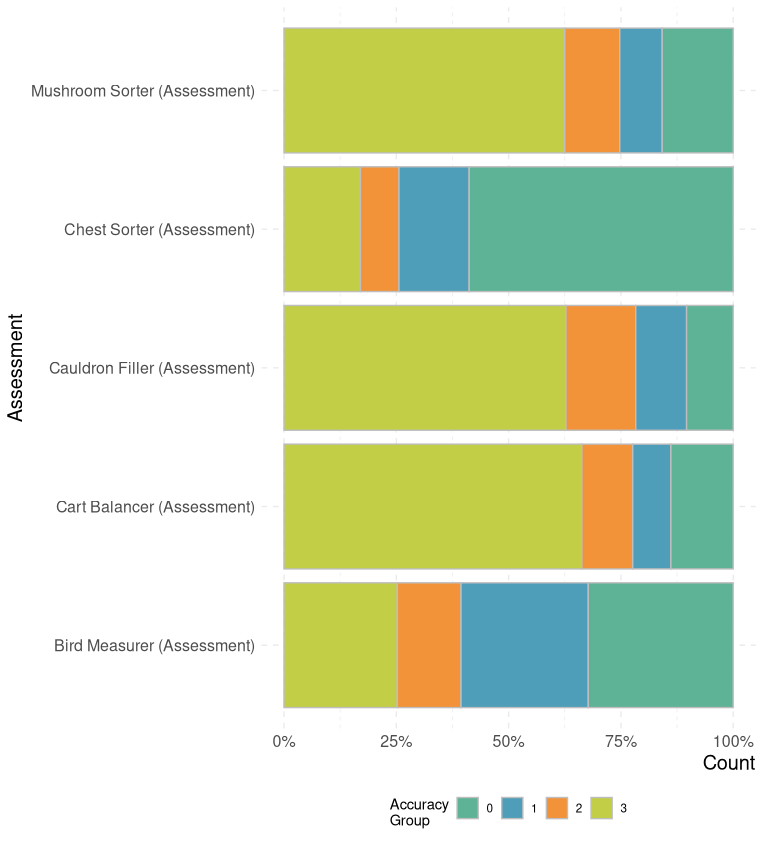
\includegraphics[width=\linewidth]{images/assessment-accuracy-by-type.png}
    \caption{Assessment accuracy by type used to build the baseline model.}
    \label{fig:assessment-accuracy-by-type}
\end{figure}

\subsection{Feature engineering}

To potentially improve the performance of proposed models it may be beneficial to firstly introduce hand-crafted features based on domain knowledge.
For this purpose the dataset was extended with fundamental summary statistics for each user such as the number of events, total, median, average and standard deviation of time spent for each type.

\subsection{Support Vector Machines}

\subsection{Comparison with XGBoost}

%------------------------------------------------

\section{Discussion}

\begin{figure*}[ht]\centering % Using \begin{figure*} makes the figure take up the entire width of the page
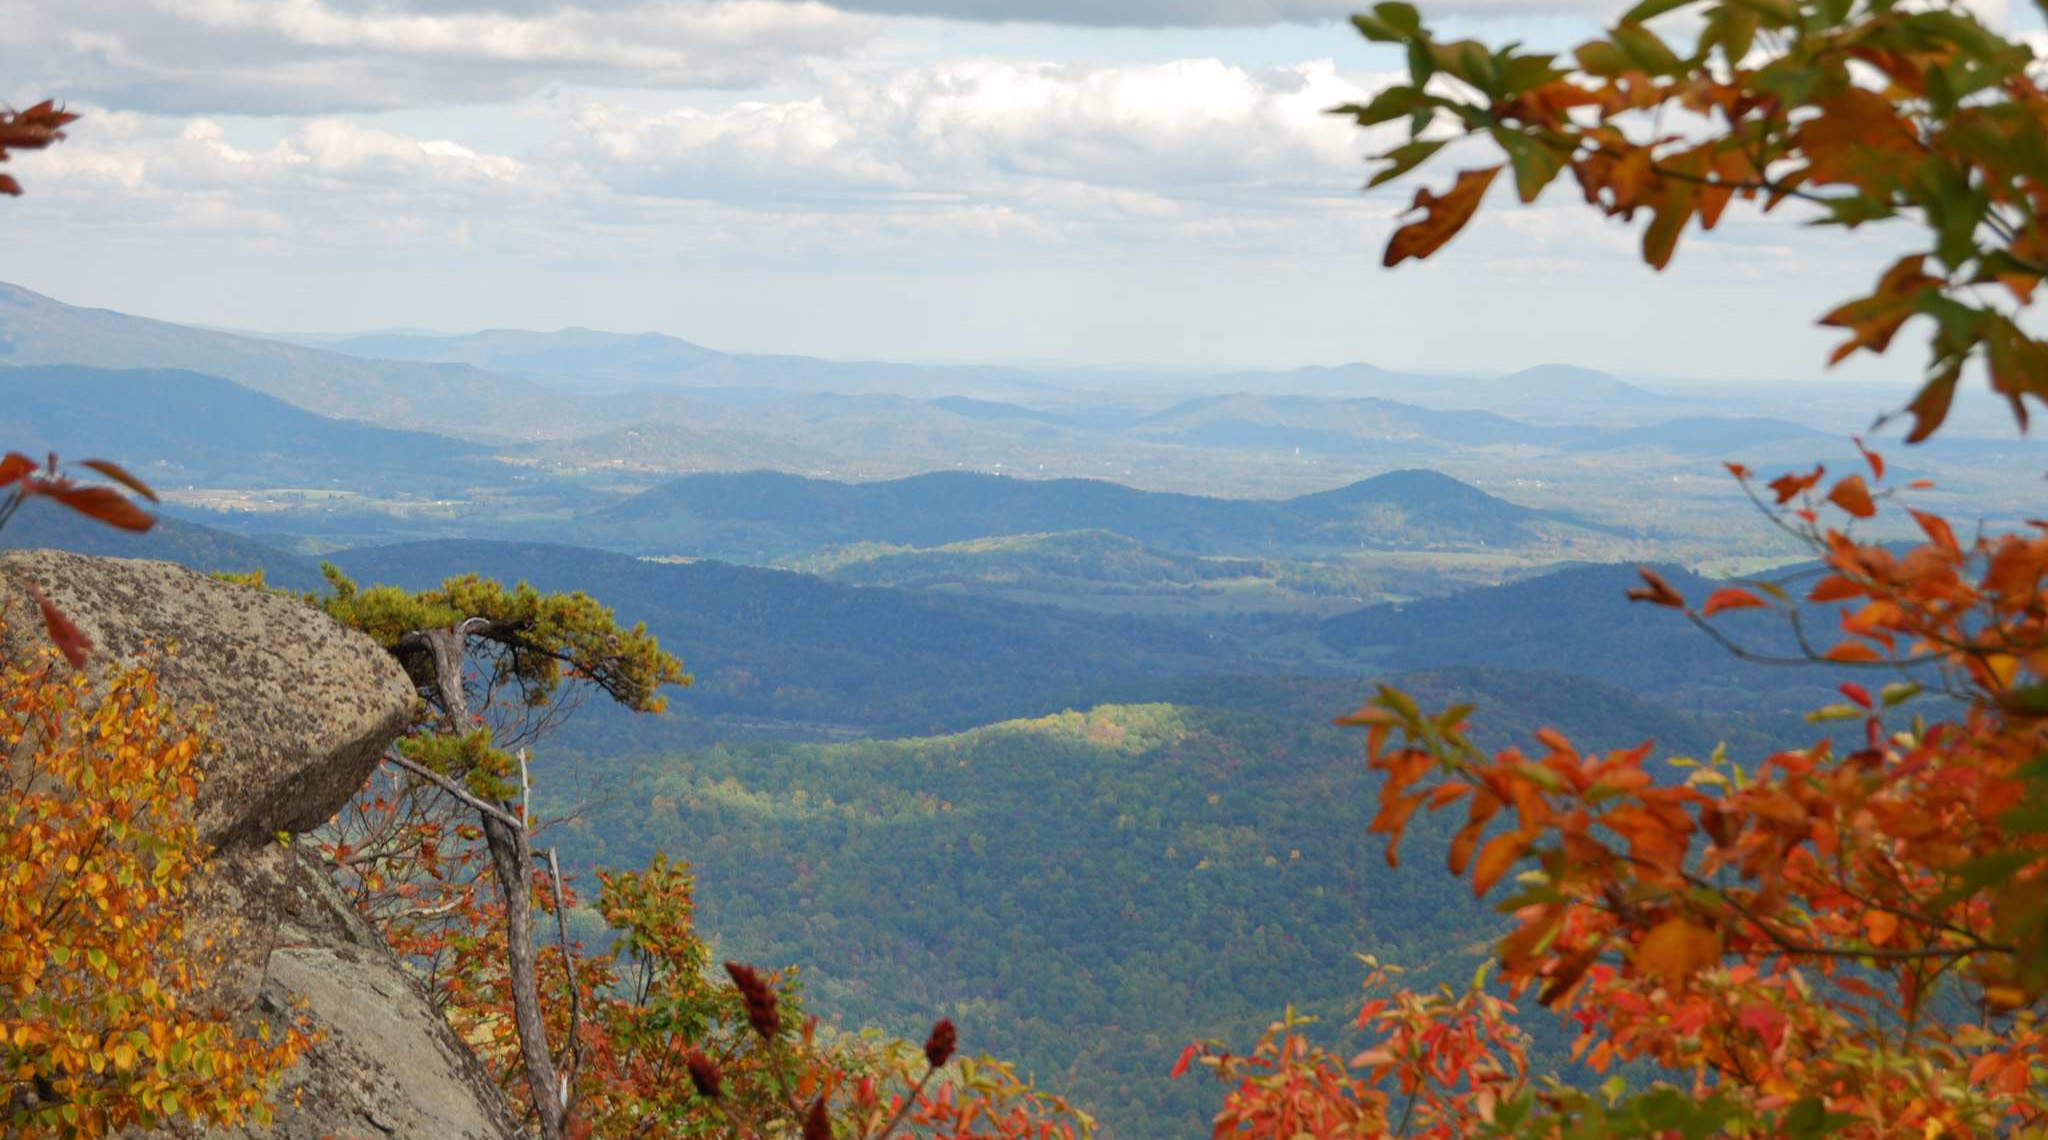
\includegraphics[width=\linewidth]{images/view}
\caption{Wide Picture}
\label{fig:view}
\end{figure*}

\lipsum[4] % Dummy text

\begin{equation}
\cos^3 \theta =\frac{1}{4}\cos\theta+\frac{3}{4}\cos 3\theta
\label{eq:refname2}
\end{equation}

\paragraph{Paragraph} \lipsum[7] % Dummy text

\begin{table}[hbt]
\caption{Table of Grades}
\centering
\begin{tabular}{llr}
\toprule
\multicolumn{2}{c}{Name} \\
\cmidrule(r){1-2}
First name & Last Name & Grade \\
\midrule
John & Doe & $7.5$ \\
Richard & Miles & $2$ \\
\bottomrule
\end{tabular}
\label{tab:label}
\end{table}

%------------------------------------------------
\phantomsection
\section*{Acknowledgments} % The \section*{} command stops section numbering

\addcontentsline{toc}{section}{Acknowledgments} % Adds this section to the table of contents

So long and thanks for all the fish~\cite{svm}.

%----------------------------------------------------------------------------------------
%	REFERENCE LIST
%----------------------------------------------------------------------------------------
\phantomsection
\bibliographystyle{unsrt}
\bibliography{report}

%----------------------------------------------------------------------------------------

\end{document}